%% Простая презентация с примером включения программного кода и
%% пошаговых спецэффектов
\documentclass{beamer}
\usepackage{fontspec}
\usepackage{xunicode}
\usepackage{xltxtra}
\usepackage{xecyr}
\usepackage{hyperref}
\setmainfont[Mapping=tex-text]{DejaVu Serif}
\setsansfont[Mapping=tex-text]{DejaVu Sans}
\setmonofont[Mapping=tex-text]{DejaVu Sans Mono}
\usepackage{polyglossia}
\setdefaultlanguage{russian}
\usepackage{graphicx}
\usepackage{listings}
\lstdefinestyle{mycode}{
  belowcaptionskip=1\baselineskip,
  breaklines=true,
  xleftmargin=\parindent,
  showstringspaces=false,
  basicstyle=\footnotesize\ttfamily,
  keywordstyle=\bfseries,
  commentstyle=\itshape\color{gray!40!black},
  stringstyle=\color{red},
  numbers=left,
  numbersep=5pt,
  numberstyle=\tiny\color{gray},
}
\lstset{escapechar=@,style=mycode}






% счетчик слайдов
\addtobeamertemplate{navigation symbols}{}{%
    \usebeamerfont{footline}%
    \usebeamercolor[fg]{footline}%
    \hspace{1em}%
    \insertframenumber/\inserttotalframenumber
}
\usepackage{graphicx}       % работа с картинками
\usepackage[export]{adjustbox}  % еще про место картинки (width,right/left])
\usepackage{multicol,caption,float, subfig} % картинки

\usepackage{multirow} % для няшных табличек      

\usepackage{hyperref} 


\begin{document}
\title{Методы машинного обучения \\в задаче предсказания погоды}
%\subtitle{предварительные результаты}
\author{Елена Волжина\\{\footnotesize\textcolor{gray}{руководитель Е.Г. Михайлова}}}
\institute{СПбГУ, мат-мех, кафедра ИАС}
\date{31 мая 2018г}
\frame{\titlepage}

\begin{frame}\frametitle{\large Введение}
\begin{itemize}
    % что мы называем погодой?
    \item Погода -- состояние нижнего слоя атмосферы % (нижней тропосферы) в определённом месте в определённое время
    
    % что её характеризует?
    \item Температура, погодное явление, влажность, давление, ветер, ...
    
    % как мы можем её измерить?
    \item Метеостанции, метеорадары, спутники
    
    % как делается прогноз?
    \item Численный прогноз погоды % Газодинамика, ур-ния Навье-Стокса описывают движение вязкой жидкости, не решены аналитически
    
    % это сложно, всего порядка 10 независимых организаций
    \item Глобальные модели: GFS, JMA, ECMWF, CMC; региональная: WRF
    
    % модели устаревают, обновлять их дико дорого, ошибки могут иметь тренды, машинное обучение!
    \item Машинное обучение: The Weather Company~(IBM), Яндекс.Погода

\end{itemize}
\end{frame}


\begin{frame}\frametitle{\large Постановка задачи}

\small{
\begin{itemize}
    \item В момент $gentime$ прогнозируем погоду \\ в момент $time$
    \item $X = \{x_i = (f^1_{i}, \cdots, f^M_i), i \in \overline{1..N}\}$, $y = \{y_i, i \in \overline{1..N}\}$
    \item $f_i$: прогнозы поставщиков, климатические данные, вспомогательные переменные
    
    \hspace\\
    
    \item \textbf{Задача 1}: для модели прогноза температуры добавить показания ближайших станций в момент $gentime$ (на 7 часов вперёд)
    \item Целевые значения -- $temperature\_delta$ % = temperature - climate\_temperature$
    
    \hspace\\
    
    \item \textbf{Задача 2}: обучить модель для предсказания интенсивности осадков (если они есть)
    \item Целевые значения -- агрегированные по времени и географии значения с метеорологических радаров
    %\item Только положительные значения

\end{itemize}

}
\end{frame}



\begin{frame}\frametitle{\large Постановка задачи}
{\small
    \begin{itemize}
        \item Градиентный бустинг над решающими деревьями

    \only<1>{\begin{figure}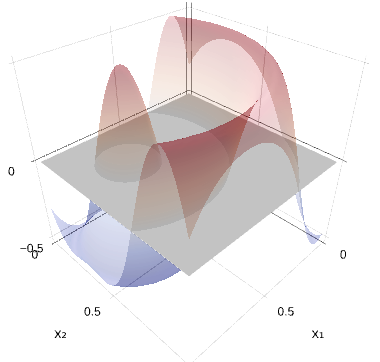
\includegraphics[width=0.4\linewidth]{images/preso_gb_left_0_contrast.png}\caption*{\footnotesize Градиентный бустинг: 0 деревьев}\end{figure}}
    \only<2>{\begin{figure}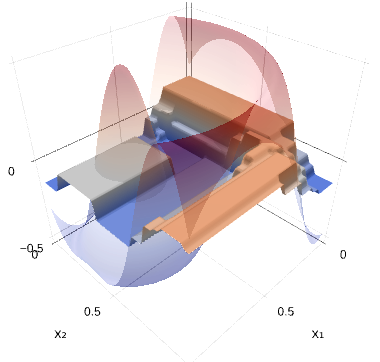
\includegraphics[width=0.4\linewidth]{images/preso_gb_left_1_contrast.png}\caption*{\footnotesize Градиентный бустинг: 1 дерево глубины 6}\end{figure}}
    \only<3>{\begin{figure}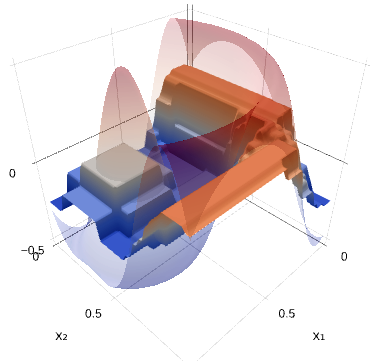
\includegraphics[width=0.4\linewidth]{images/preso_gb_left_2_contrast.png}\caption*{\footnotesize Градиентный бустинг: 2 дерева глубины 6}\end{figure}}
    \only<4>{\begin{figure}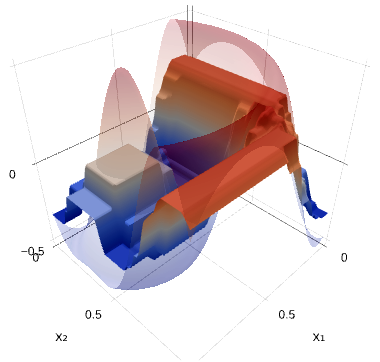
\includegraphics[width=0.4\linewidth]{images/preso_gb_left_3_contrast.png}\caption*{\footnotesize Градиентный бустинг: 3 дерева глубины 6}\end{figure}}
    \only<5->{\begin{figure}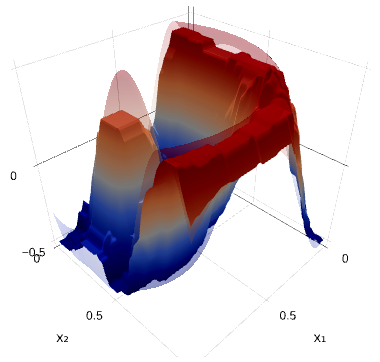
\includegraphics[width=0.4\linewidth]{images/preso_gb_left_10_contrast.png}\caption*{\footnotesize Градиентный бустинг: 10 деревьев глубины 6}\end{figure}}

        \item<6-> В Яндексе: Matrixnet, CatBoost
        
        \item<7-> Метрика: $RMSE(y, \hat{y}) = \sqrt{\frac{\sum^{n}_{i=1}{(y_i - \hat{y_i})^2}}{n}}$
    \end{itemize}
    
    {\tiny \color{gray} \url{http://arogozhnikov.github.io/2016/06/24/gradient_boosting_explained.html}}

}
\end{frame}

%%%%%%%%%%%%%%%%%%%%%%%%%%%%%%%%%%%%%%%
%%%%%%%%%%% ТЕМПЕРАТУРА %%%%%%%%%%%%%%%
%%%%%%%%%%%%%%%%%%%%%%%%%%%%%%%%%%%%%%%

\begin{frame}\frametitle{\large Эксперименты с температурой: начальное решение}

Модели, обученные на всех краткосрочных горизонтах

\begin{figure}
\centering
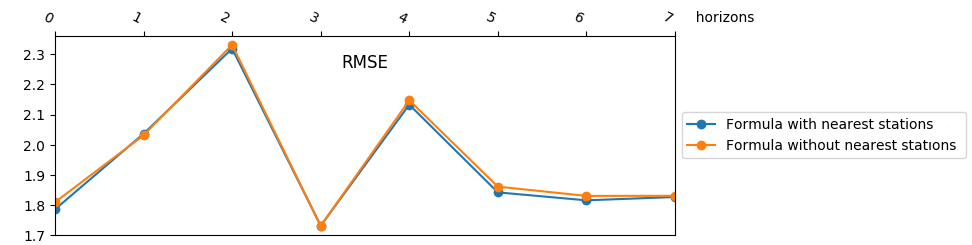
\includegraphics[width=\linewidth]{images/pic1_metrics_initial.png}
\end{figure}

% $fact1\_temperature\_delta$ на 151 месте из 250
\end{frame}



\begin{frame}\frametitle{\large Эксперименты с температурой: первые N часов}

\begin{figure}\centering
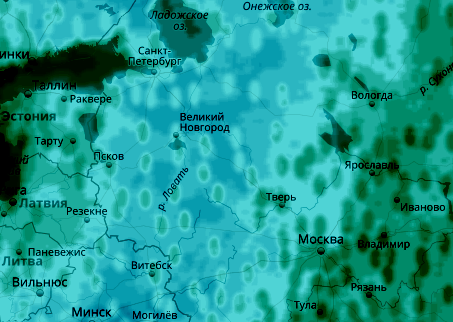
\includegraphics[width=0.9\linewidth]{images/pic2_map_contrast.png}
\end{figure}
% $fact1\_temperature\_delta$ на 5 месте по эффекту, наравне с прогнозами температуры от поставщиков
\end{frame}



\begin{frame}\frametitle{\large Эксперименты с температурой: сглаживание}
\setlength\parindent{24pt}

\begingroup
\setlength\abovedisplayskip{0pt}

\begin{multline*}
smoothed\_fact\_temperature\_delta := \\\left\{
    \begin{array}{ll}
      fact \cdot (1 - \frac{dist}{max\_distance}) + forecast \cdot \frac{dist}{max\_distance},
      \\\indent \text{     if }dist \le max\_distance  \\
      forecast, \text{ if } dist > max\_distance
    \end{array}
  \right.,
\end{multline*}
\endgroup

{\scriptsize 
    \indent где $fact$ -- исходное значение с одной из ближайших станций, \\
    \indent $dist$ -- расстояние до неё, $forecast$ -- прогноз поставщика
}

\begin{figure}
\centering
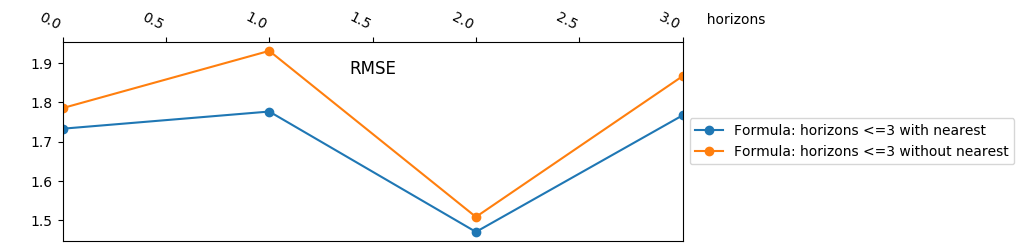
\includegraphics[width=\linewidth]{images/pic3_metrics_final.png}
\end{figure}

% Сглаженные температуры с двух ближайших станций оказались на 1 и 4 местах по влиянию на ответ модели.
% пятен нет
% это в проде!
\end{frame}




%%%%%%%%%%%%%%%%%%%%%%%%%%%%%%%%%%%%%%%
%%%%%%%%%%%%%% ОСАДКИ %%%%%%%%%%%%%%%%%
%%%%%%%%%%%%%%%%%%%%%%%%%%%%%%%%%%%%%%%

\begin{frame}\frametitle{\large Эксперименты с осадками}

\begin{figure}\centering
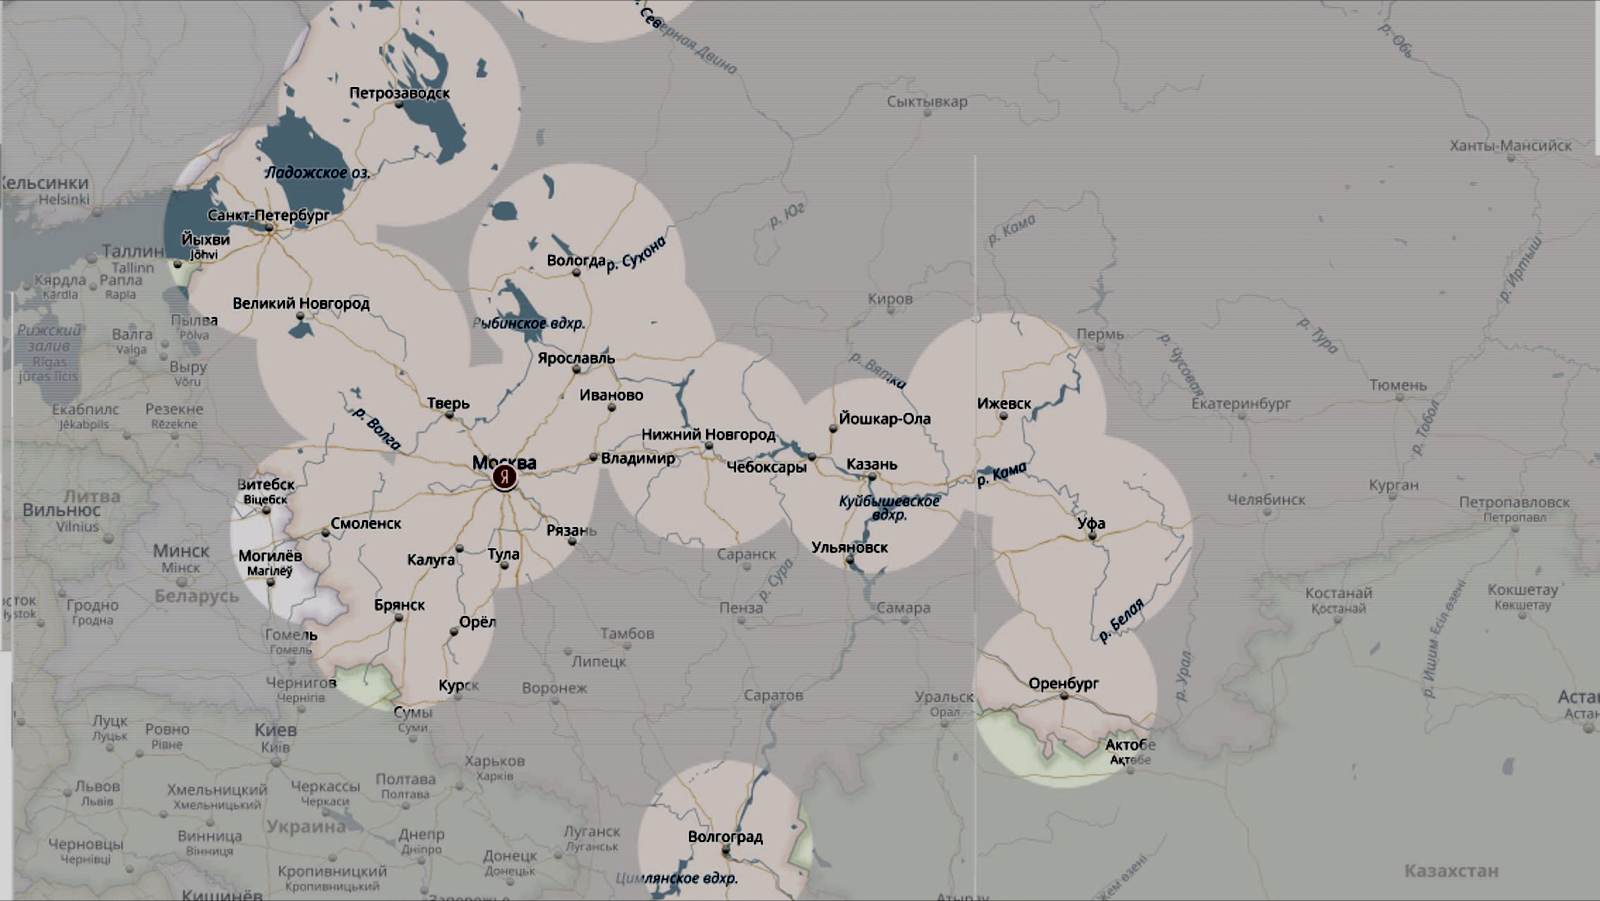
\includegraphics[width=0.9\linewidth]{images/pic5_radars_map_contrast.png}
\end{figure}
% радары лучше станций

Обработка радаров:
\begin{itemize}
    \item склейка   % не я
    \item фильтрация
    \item агрегация
\end{itemize}

\end{frame}


\begin{frame}\frametitle{\large Эксперименты с осадками: начальное решение}

\begin{itemize}
    \item один месяц, точки станций
    \item агрегация по времени за час и по географии в радиусе 3 километров
    \item пороги для отсечения шумовых значений
\end{itemize}

Результаты неудовлетворительные, по RMSE модель не выигрывает прогнозы поставщиков, быстрое переобучение.

\end{frame}



\begin{frame}\frametitle{\large Эксперименты с осадками: проверки данных}

\begin{itemize}
    \item согласованность радаров: предыдущий час в признаки
    \item согласованность поставщиков: предсказывание одного по другим
    \item упрощение задачи: классификация
\end{itemize}


\end{frame}




\begin{frame}\frametitle{\large Эксперименты с осадками: улучшение сбора данных}

\begin{itemize}
    \item три месяца, точки сетки
    \item агрегация по времени за три часа и по географии в радиусе 30 километров
    \item дисбаланс в значениях: \\
    \begin{itemize}
        \item логарифмирование
        \item отдельно $(0, 1]$ и $(1, +\infty)$
        \item искусственное балансирование данных
    \end{itemize}
\end{itemize}

CatBoost 

\end{frame}




\begin{frame}\frametitle{\large Эксперименты с осадками: результаты}

\small{

\begin{table}[H]
  \centering
  \begin{tabular}{ l | r | r }
     & model RMSE & provider RMSE \\ 
     \hline
    simple regression, any target &  0.5386  &  0.8431 \\ 
    log precipitation, any target &  0.5482  &  0.8431 \\ 
    simple regression @ $(0, 1]$  &  0.1890  &  0.7165 \\ 
    log precipitation @ $(0, 1]$  &  0.1898  &  0.7165 \\ 
  \end{tabular}
  \caption*{обычная обучающая выборка}
  \label{table_simple_pool}
\end{table}

\begin{table}[H]
  \centering
  \begin{tabular}{ l | r | r }
     & model RMSE & provider RMSE \\ 
    simple regression             &  1.6231  &  1.8527 \\ 
    log precipitation             &  1.6977  &  1.8527 \\ 
    simple regression + weights   &  1.6695  &  1.8527 \\ 
    log precipitation + weights   &  1.7330  &  1.8527 \\ 
  \end{tabular}
  \caption*{сбалансированная обучающая выборка}
  \label{table_balanced_pool}
\end{table}


}
\end{frame}



%%%%%%%%%%%%%%%%%%%%%%%%%%%%%%%%%%%%%%%
%%%%%%%%%%% РЕЗУЛЬТАТЫ %%%%%%%%%%%%%%%%
%%%%%%%%%%%%%%%%%%%%%%%%%%%%%%%%%%%%%%%



\begin{frame}\frametitle{\large Заключение}

Улучшение прогнозов температуры
\begin{itemize}
    \item данные с ближайших станций наиболее полезны первые 3 часа
    \item потребовалось сглаживание
    \item модель используется в Яндекс.Погоде
\end{itemize}

\\\vspace\\\hspace\\

Прогноз интенсивности осадков
\begin{itemize}
    \item агрегация данных с радаров
    \item модель готова для использования
\end{itemize}


\end{frame}



\end{document}